\documentclass[11pt,a4paper]{article}
\usepackage[margin=2.4cm]{geometry}
\usepackage[T1]{fontenc}
\usepackage[utf8]{inputenc}
\usepackage{lmodern}
\usepackage{amsmath}
\usepackage{graphicx}
\usepackage{booktabs}
\usepackage{tabularx}
\usepackage{natbib}
\usepackage[hidelinks]{hyperref}
\usepackage{xcolor}
\setlength{\parskip}{4pt}
\setlength{\parindent}{0pt}
% A claim id in the repository's ledger (docs/claims.yaml): every number that carries one is checked
% against a committed artifact by scripts/claims.py, and the marker is how a reader finds the check.
\newcommand{\claim}[1]{{\scriptsize\textsf{\textcolor{gray}{[#1]}}}}
\newcommand{\pkg}{\texttt{olmoearth\_inferenceX}}
\newcommand{\code}[1]{\texttt{#1}}

\title{\pkg: confidence-based review, comparison and accuracy estimation for Earth-observation classification maps\\[6pt]
\large Technical report, version 1.3.0}
\author{Ziming Qi\\[2pt] \small \url{https://github.com/2imi9/olmoearth_inferenceX}\\[-1pt]
\small \url{https://olmoearth-inferencex.readthedocs.io}}
\date{24 September 2026}

\begin{document}
\maketitle

\begin{abstract}
This report describes \pkg, a Python package for assessing classification maps from Earth-observation models, and
the record behind it. Without labels, the package ranks a map's windows for review by the model's confidence margin,
explains each flagged window by label-free cues, and compares two maps with regard to their dates. With a labelled
sample, it estimates error rate and per-class accuracy with design-based intervals and certifies a high-confidence zone
whose error rate is bounded with a stated probability. On all 24 tasks
of the model authors' published embedding suite that define a margin, the margin ranks the model's errors better than
the best control that does not use the model, and under ten probe seeds it does so on at least 75\% of the tasks of
each of the suite's sixteen encoders. A simple random sample of 300 windows gives a nominal 95\% interval that covers
the true error rate on 0.933 to 0.961 of simulated draws on seven segmentation tasks; labelling 19 tiles of 16 windows
and applying the independent-sample formula covers on 0.506 to 0.777 of draws on six of them. The certified zone met
its guarantee on all 112 graded cells. The record comprises 86 experiment scripts and 204 ledger claims, each checked
against a committed artifact, and reports failed predictions as failed.
\end{abstract}

\section{Introduction}

A classification map from an Earth-observation model is usually applied where no reference labels exist. This report addresses three questions: which windows to review first when only a
fraction can be checked; how two maps of one area differ, when they come from different crops, backbones, sensors,
encoders, training states or dates; and, once some windows are labelled, how wrong the map is, how accurate each class
is, and which part of it can be used with a stated error bound.

\pkg{} ranks $4\times4$-pixel windows by the model's confidence margin with label-free cues (Section~\ref{sec:ranking}),
compares two maps with regard to their dates (Section~\ref{sec:compare}), estimates error rates and per-class accuracies
from a labelled sample (Section~\ref{sec:estimate}), and certifies a zone of the most confident windows
(Section~\ref{sec:zone}). It reads arrays and rasters and loads no model. In the evaluation the label-free readings are graded against labels and never fitted
to them \claim{labels-grade-never-train}.

\paragraph{Relation to prior work.} No component is new in isolation. Risk-coverage evaluation comes from selective
classification \citep{chow1970,geifman2017,geifman2019}, softmax confidence as the error-detection baseline from
\citet{hendrycks2017} and \citet{jaeger2023}, and the margin from margin sampling \citep{scheffer2001,lewis1994}; related
measures are \citet{rottmann2020} and \citet{meyer2021}. The estimators follow design-based map-accuracy practice
\citep{olofsson2014,stehman2019}, and the certified zone follows risk control by exact tests
\citep{bates2021,angelopoulos2021}. This work applies them to Earth-observation maps at the window level and tests the
known signals against the model's confidence and against controls that do not use the model.

\section{Methods}
\label{sec:methods}

\subsection{Windows, the confidence signal and the ranking}
\label{sec:ranking}

Pixels are grouped into windows of $4\times4$ pixels, the unit of ranking, comparison and estimation. A window's
decision is the majority class of its pixels, and a tie goes to the class whose voting pixels are more
confident. For a pixel with logits $z_{(1)} \ge z_{(2)} \ge \dots$, the confidence is the margin
\begin{equation}
  m = z_{(1)} - z_{(2)},
\end{equation}
and for a binary logit map the absolute logit $|z|$. For a probability map it is the top class probability, which ties
where probabilities saturate, so logits are preferred. The option \code{form="top1"} ranks a multi-class logit map by
$1 - p_{(1)}$ computed from the logits without ties. A window's confidence $m(w)$ is the pixel confidence averaged over
the window, and its suspicion is $\sigma(w) = -m(w)$.

A window is a boundary window when any of its eight neighbours has a different decision. The confidence order sorts
windows by decreasing suspicion; the boundary-first order takes the boundary windows first, each group by suspicion.
The review set at budget $b$ is the first $\max(1, \mathrm{round}(bN))$ of the $N$ valid windows. Each flagged window
carries the cues it satisfies: boundary, low confidence (the least confident fifth), tiling instability (a changed
decision under a two-pixel crop shift) and, for water maps, spectral ambiguity. A cue's enrichment, its share among
error windows over its share among correct windows, is quoted as measured on labelled data; since version 1.3.0 the
boundary cue is quoted with the range measured on the suite and the map's own boundary prevalence.

\begin{figure}[t]
\centering
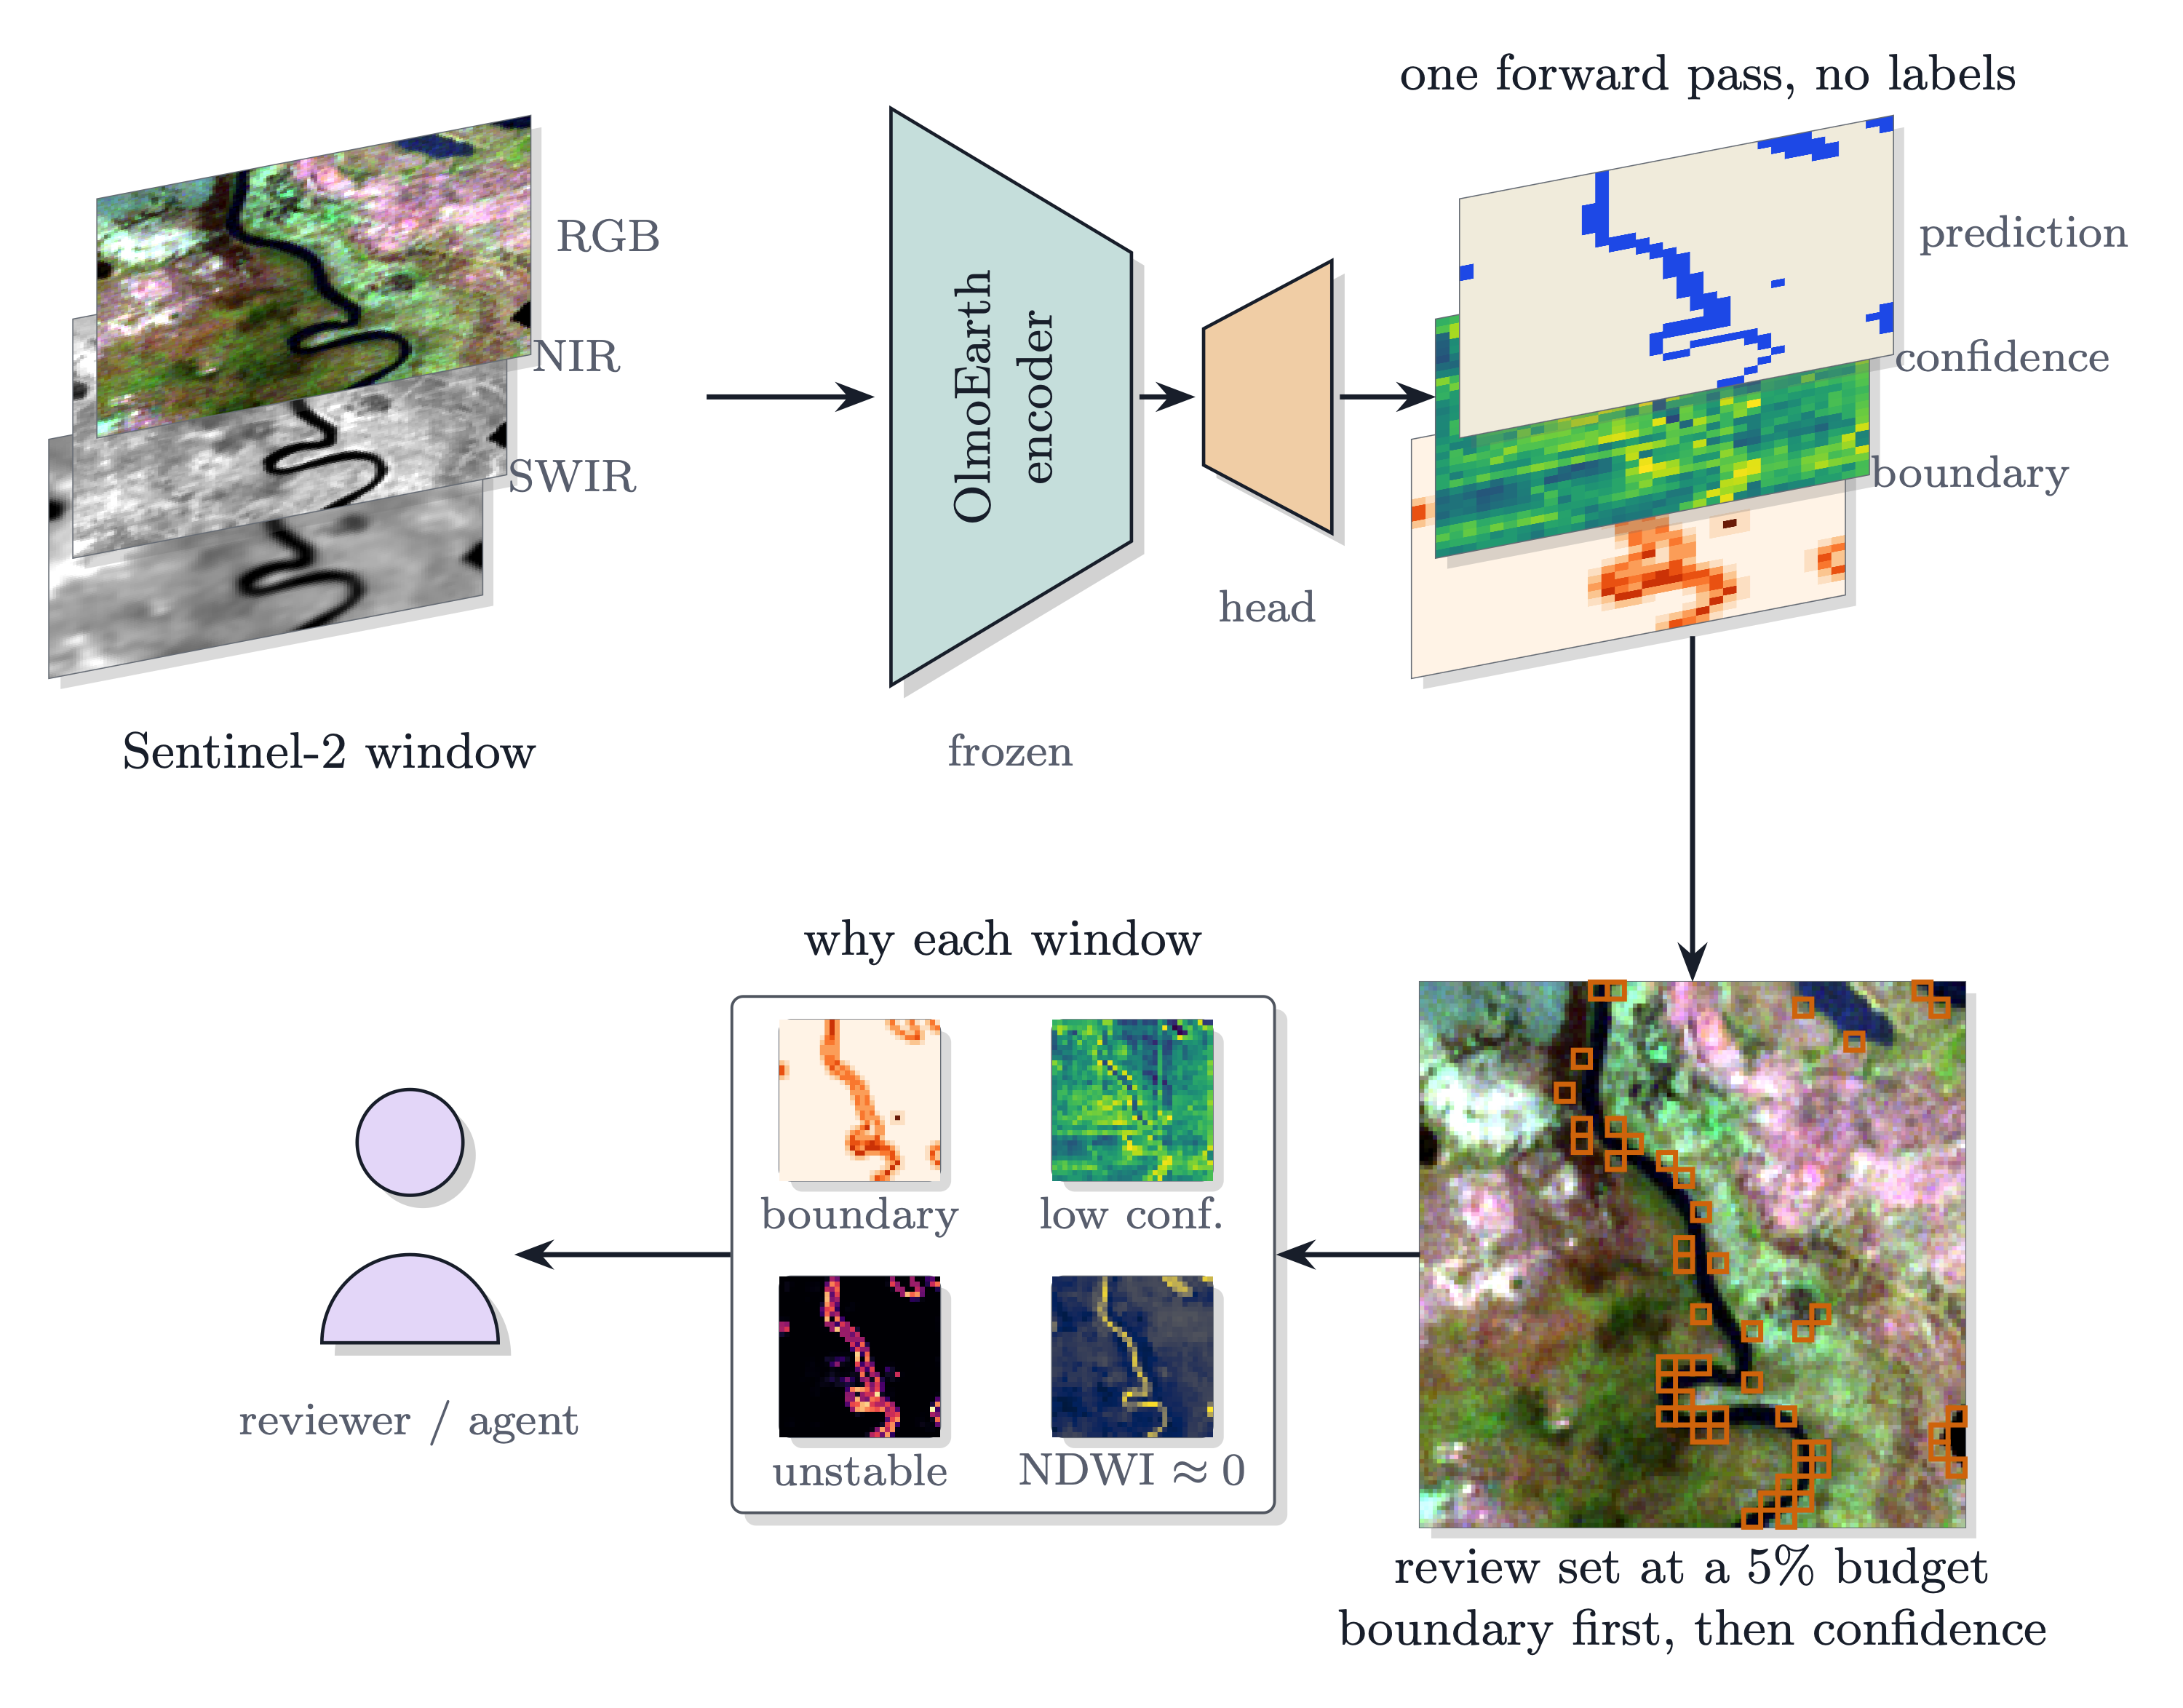
\includegraphics[width=0.92\linewidth]{../docs/figures/pipeline.png}
\caption{One scene through the label-free assessment: Sentinel-2 bands, the frozen OlmoEarth encoder and a task head,
the prediction with its confidence and boundary layers, the review set at a 5\% budget, and the cues per flagged window.}
\label{fig:pipeline}
\end{figure}

\subsection{Comparison of two maps}
\label{sec:compare}

For hard window decisions $A$ and $B$ of two maps on one grid, over the windows $V$ both predict, the package reports
without labels the disagreement rate $D = |\{w \in V : A(w) \neq B(w)\}| / |V|$, pooled and per group (tile, event or
zone), the enrichment of each cue among differing windows, and the $\phi$ coefficient between two disagreement masks,
which measures whether two differences occupy the same windows. A rate is read against the reseed floor, the rate at
which refitting the head with another seed changes decisions. With labels, a separate block adds the cross-tabulation
of the two error maps and the share of differing windows on which each map matches the label.

Each map may carry the date or period it represents. At one time a difference implies an error in at least one map;
across times it may be change on the ground, and the package then grades which map is right only when the labels' date
is given, reporting which map the labels match in time; with one date stated, grading is refused. Without labels the
package does not decide which map is right.

\begin{figure}[t]
\centering
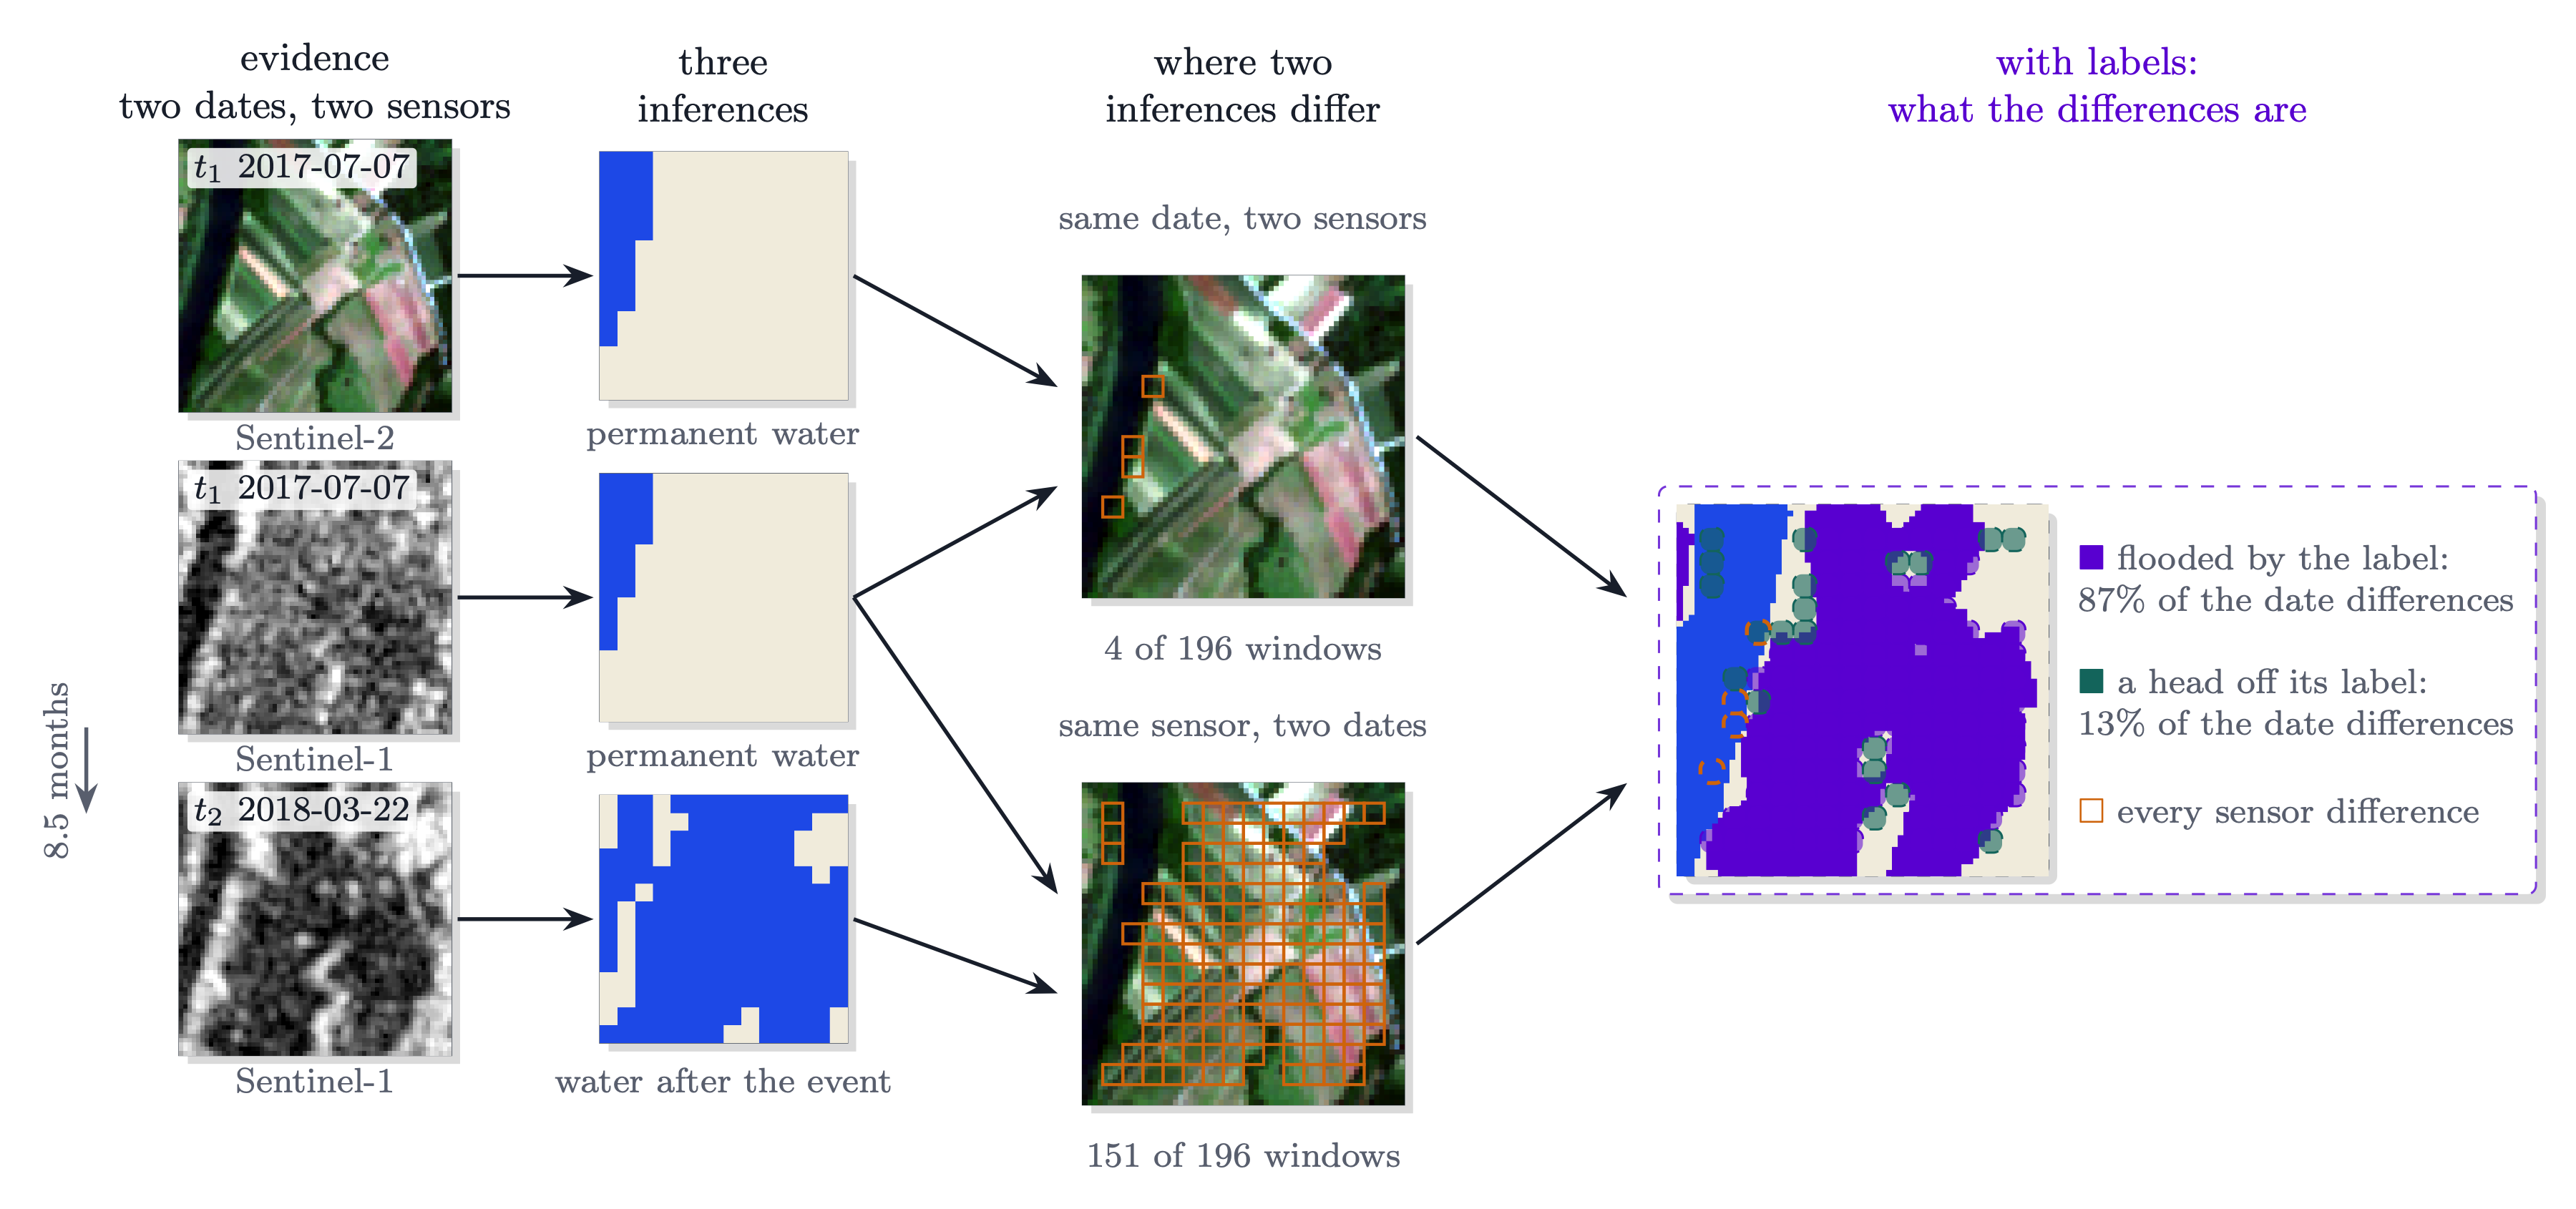
\includegraphics[width=0.92\linewidth]{../docs/figures/compare.png}
\caption{Four dated inputs of one GEOID-Flood chip, each read on identical windows: the same-period and same-sensor
differences on the scene, with the comparison against labels shown separately.}
\label{fig:compare}
\end{figure}

\subsection{Design-based estimation}
\label{sec:estimate}

Let the map have $N$ valid windows, $e_i = 1$ where the map's class differs from the reference class, and
$\theta = N^{-1}\sum_i e_i$. A reviewer labels $B$ windows under one of three designs.

\textbf{Confidence-stratified design (default).} Five strata are cut at the quintiles of the margin, with sizes $N_h$
and weights $W_h = N_h/N$. The budget follows Neyman's allocation, which minimises the variance of the stratified
estimate at a fixed budget,
\begin{equation}
  n_h = B \, \frac{N_h S_h}{\sum_j N_j S_j}, \qquad S_h \approx \sqrt{q_h (1 - q_h)},
\end{equation}
where $q_h$ is the mean of $1 - p_{(1)}$ in stratum $h$, floored at 0.02, and each stratum receives at least two
labels. With $p_h$ the error share among stratum $h$'s labels and $f_h = n_h/N_h$,
\begin{equation}
  \hat\theta = \sum_h W_h \, p_h, \qquad
  \hat v = \sum_h W_h^2 (1 - f_h) \, \frac{p_h (1 - p_h)}{n_h - 1},
\end{equation}
both unbiased under stratified sampling without replacement, with Wilson's interval at the effective sample size
$\hat\theta(1-\hat\theta)/\hat v$ (Korn and Graubard, 1998).

\textbf{Simple random design.} The sampled error count $k$ is hypergeometric, and the interval for $\theta = K/N$ holds
every $K$ whose two tail probabilities at $k$ both exceed 0.025, widened if needed to contain $k/n$; its coverage is at
least 95\% for every $(N, K, n)$.

\textbf{Tile design.} With 16 windows labelled in each of $t$ tiles, the estimate is the ratio
$\hat\theta = \sum_i n_i \bar y_i / \sum_i n_i$ with ultimate-cluster variance
$\sum_i n_i^2 (\bar y_i - \hat\theta)^2 / (t(t-1)\bar n^2)$, reported beside the independent-sample interval; its
variance ratio to simple random sampling is the design effect.

\textbf{Review-set check.} Labelling the review set gives the error share $\mathrm{capture}(b)\,\theta/b$, where
$\mathrm{capture}(b)$ is the set's share of all errors. Windows labelled without a design are accepted as a random
sample only if their mean suspicion percentile lies within four standard deviations of 0.5.

\textbf{Per-class accuracy.} With map class $m$ and reference class $r$, the user's accuracy is
$\mathrm{UA}_c = \#\{m{=}c, r{=}c\}/\#\{m{=}c\}$, the producer's accuracy $\mathrm{PA}_c = \#\{m{=}c, r{=}c\}/\#\{r{=}c\}$
and the error-adjusted share $A_c = \#\{r{=}c\}/N$. Under a random sample $\mathrm{UA}_c$ has the exact interval, and
$A_c$ and $\mathrm{PA}_c$ \citep{olofsson2014} have Wilson intervals at the effective sample size; under the confidence
design each is a ratio of Horvitz--Thompson (inverse-probability-weighted) totals with a linearised variance. Warnings
mark classes with fewer than 30 labels, thin or near-census sampling, one to four sampled errors, or no prediction.

\subsection{The certified zone}
\label{sec:zone}

Windows are ordered by decreasing margin, ties by index; the zone at coverage $c$ is the first $n_c =
\mathrm{round}(cN)$ windows, and its risk $R(c)$ is the error rate inside it, for $c \in \{0.05, 0.10, \dots, 1.00\}$.
From a simple random sample of $B$ labels, of which $b_c$ fall in the zone and $k_c$ of those are errors, the exact
one-sided p-value against $R(c) > \alpha$ is
\begin{equation}
  p_c = P(X \le k_c), \qquad X \sim \mathrm{Hypergeom}\bigl(n_c,\ \lfloor \alpha n_c \rfloor + 1,\ b_c\bigr).
\end{equation}
A rule returns a coverage $\hat c$ or no zone and is valid when $P(R(\hat c) > \alpha) \le \delta$ over the draw. The
prefix rule \citep{bates2021} accepts coverages from the smallest upward while $p_c \le \delta$, valid when $R(c)$ does
not decrease with $c$; the Bonferroni rule \citep{angelopoulos2021} accepts every coverage with $p_c \le \delta/J$ over
$J$ levels and assumes nothing. Even without errors, a zone needs $\lceil \ln\delta / \ln(1-\alpha) \rceil$ labels, 45 at
$\alpha = 0.05$ and 255 at $\alpha = 0.009$ for the default $\delta = 0.1$; the package refuses budgets that cannot
certify the level and non-random samples, and certifies nothing outside the zone.

\section{Evaluation protocol}
\label{sec:protocol}

\subsection{Units, statistics and controls}

The graded unit is the window on segmentation maps and the sample on classification tasks. With $n$ units and
$k$ errors, the selective risk at a coverage is the error rate among the least suspect units kept; AURC is
its mean over the $n$ coverage levels, in expectation over orderings of tied units. The perfect ranking has
$\mathrm{AURC}_{\mathrm{o}} = n^{-1}\sum_{i=1}^{n} \max(0, i - (n - k))/i$, the excess AURC is
$\mathrm{AURC} - \mathrm{AURC}_{\mathrm{o}}$ \citep{geifman2019}, and since a random ranking scores $e = k/n$, a reading
takes the share $1 - \text{E-AURC}/(e - \mathrm{AURC}_{\mathrm{o}})$ of the ranking headroom. The capture at budget $b$
is the review set's share of all errors, reported beside its ceiling $\min(1, b/e)$. For a fixed error set AUGRC
\citep{traub2024} is a decreasing affine function of the failure AUROC. Readings are compared by one-sided exact sign
tests over independent groups (tiles, events, regions, tasks), design-weighted \citep{olofsson2014} where the reference is
a probability sample.

A candidate signal is supported only if it beats both the model's confidence and a control that does not use the
model, and the margin must beat the control. On imagery the controls are pixel statistics such as a water index; on
the published suite, whose imagery is not released, they are a sample's embedding distance from the training mean and
the rarity of its predicted class.

\subsection{Kinds of reference}

Table~\ref{tab:refs} lists the labelled testbeds. The OlmoEarth paper's embedding suite \citep{herzog2025} adds 24
tasks with splits fixed by the model authors; as every unit is labelled, estimators are graded on it over 2,000
simulated draws of 300 labels.

\begin{table}[h]
\centering\small
\begin{tabularx}{\linewidth}{lX}
\toprule
Origin of the reference & Testbeds \\
\midrule
people interpreting the imagery & Sen1Floods11 \citep{bonafilia2020}, GEOID-Flood (Copernicus EMS) \citep{chiriaco2026}, WorldFloods~v2 \\
another model's output & DFC2020 \citep{yokoya2020}, an iterated random forest \\
experts annotating a product & Dynamic World \citep{brown2022}, 409 tiles \\
surveyors in the field & LUCAS Copernicus 2022 \citep{dandrimont2021} \\
farmers' declarations & EuroCrops \citep{schneider2023}, labelled in both years \\
\bottomrule
\end{tabularx}
\caption{Labelled testbeds by origin of the reference.}
\label{tab:refs}
\end{table}

\subsection{Preregistration, the claim ledger and corrections}
\label{sec:protocol-ledger}

Each experiment states its predictions and falsification conditions before it runs, with dated amendments. The repository holds 86 experiment scripts named \code{expNN\_*.py}, covering 82 experiment
numbers from exp01 to exp85. The ledger \code{docs/claims.yaml} holds 204 claims, each with a statement, status,
artifacts and an executable check; 62 are supported, 67 measured, 29 mixed, 44 rejected and 2 superseded, and
\code{scripts/claims.py stale} currently flags only the two superseded ones. After an audit on 23 September 2026 found
that 138 of the then 167 checks read a result back from its own artifact, second routes were added, and 60 of the 204 claims now name a
\code{crosscheck} test that recomputes the statistic; exp79 and exp84 were recomputed by an independent route before recording.

Corrected results appear in their current form. exp78's cluster-corrected arm is now the ratio estimator, which
restores coverage where tiles are of equal size and not on MADOS, and the earlier statement to the contrary was
withdrawn. The
finite-population Wilson interval is now the score inversion at the effective size $n(N-1)/(N-n)$, after the earlier
form excluded a true rate of 0.010 whenever a 100-window class's single error was sampled in 30 labels. exp70's third
prediction, reported at $p = 6.9\times10^{-15}$ from 144 task pairs treated as independent, has $p = 0.0054$ by a
rank-sum test over tasks and still holds. exp54's cross-encoder $\phi$ block was withdrawn.

\section{Results}
\label{sec:results}

\subsection{Ranking on the labelled testbeds}

The model's own confidence is the best single label-free error ranker on the AWF points, the fine-tuned model and the
multi-region Sen1Floods11 test split, under both backbones and both window designs, leading or tying
\claim{confidence-best-single-signal}. On the median of 45 GEOID-Flood areas of interest, the 5\% of windows it flags
hold 88\% of the permanent-water and 64\% of the post-event water errors, 17.5 and 12.8 times a random 5\%
\claim{geoid-capture-effect-size}. On Sen1Floods11 Bolivia, one flood event, the NDWI control ranks the errors as well
as confidence under OlmoEarth v1 and better under v1.2 Base \claim{bolivia-ndwi-exception}; over the GEOID-Flood areas
the exception rate is one activation in nine \claim{geoid-exception-rate}; and after fine-tuning, the model's confidence
beats the NDWI control on Bolivia under both backbones \claim{finetune-dissolves-bolivia-exception}.

\subsection{The published embedding suite}
\label{sec:res-suite}

Of 25 suite tasks, 24 define a margin. On all 24 and all 14 distinct sources, the margin ranks the errors of
OlmoEarth Base's probe better than the best no-model control, with leads of 0.0157 to 0.2278 of excess AURC over
6,435,473 units and accuracies from 0.333 to 0.979 (sign test $p = 6\times10^{-8}$) \claim{suite-margin-wins-every-task},
including all six GEO-Bench tasks \citep{lacoste2023} \claim{suite-holds-in-both-families}. Under ten probe seeds the
lead stays positive on all 24, the smallest being $+0.0017$ on CropHarvest Togo Sentinel-1
\claim{exp79-base-margin-wins-under-every-seed}. The margin beats a five-seed ensemble \citep{lakshminarayanan2017} on 22
of 24 tasks and the nearest-neighbour \citep{sun2022} and Mahalanobis \citep{lee2018} distances on 24 of 24
\claim{suite-margin-beats-the-strong-alternatives}; only the ensemble beats it, on EuroSAT and AWF Landsat
\claim{suite-alternatives-clear-the-control-and-still-lose}.

Under the fifteen other encoders of the suite (eight families outside OlmoEarth and the OlmoEarth size series), the
margin wins on 322 of 332 (encoder, task) pairs, every encoder on at least 90.5\% of its tasks
\claim{suite-holds-under-every-encoder}; under each of ten seeds it wins on at least 75\% of the tasks of all sixteen
encoders, the lowest share 0.875 \claim{exp79-headline-holds-under-every-seed-on-every-encoder}. Its 122 failures over the 150 encoder-seeds
of the fifteen lie on the three 306-unit CropHarvest Togo tasks or on Nandi Sentinel-1 at a probe accuracy of at most
0.40 \claim{exp84-losses-are-small-or-badly-fitted-tasks}, and the per-encoder sign test survives a Holm correction at
every seed \claim{exp84-bar-survives-holm}. The margin takes a median 0.68 of the ranking headroom
\claim{margin-takes-two-thirds-of-the-ranking-headroom}; across encoders the median share runs from 0.551 to 0.693, and
its standard deviation between tasks is 2.8 times that between encoders within a task
\claim{the-ranking-ceiling-is-the-tasks-not-the-encoder}.
The best encoder is OlmoEarth Large or Base under every seed, so the record names a set of leading encoders
\claim{exp79-encoder-ordering-stable-as-a-set}. One minus the top probability ranks errors better than the margin on 14
of 16 multi-class tasks, by a median 0.0006 of excess AURC \claim{top1-beats-the-margin-on-multiclass}, and by AUROC,
hence by AUGRC, the margin beats the best control on 23 of 24 tasks \claim{augrc-leaves-the-suite-result-standing}.

\subsection{References produced independently of this project}

On Dynamic World's 409 expert-annotated tiles, the margin of the product's published probabilities ranks its errors better than a control
that uses neither imagery nor probabilities, excess AURC 0.0637 against 0.1120 \claim{dw-margin-ranks-a-production-model};
one minus the top-1 probability ties on 23.4\% of windows and the margin on 3.6\% \claim{dw-margin-beats-naive-confidence}.
On LUCAS, where a surveyor observed the point, the margin's design-weighted excess AURC is 0.1468 against 0.2421 for the
best inference-time control \claim{lucas-ranking-survives-ground-observation}. On EuroCrops it beats the best control in all three countries and on
all but four of 146 grid cells \claim{eurocrops-ranking-holds-on-declarations}, and on DFC2020 it beats the NDWI control
on all three sensor arms \claim{dfc2020-margin-beats-pixel-control}.

\subsection{Explanation cues and review order}
\label{sec:res-cues}

On Bolivia hand labels, 75\% of error windows lie on a prediction boundary against 21\% of correct windows
\claim{errors-sit-on-boundaries}, and 95\% of error windows carry at least one measured cue
\claim{explanation-cues-cover-errors}. The boundary-first order captures more errors than the confidence order at 5\% and
10\% there and not at 20\% \claim{boundary-first-review-order}. Elsewhere it wins at 5\% on a minority of GEOID-Flood
events \claim{geoid-boundary-first-minority}, and on the suite's Sen1Floods11 split it captures fewer errors at 10\% and
20\% (0.415 against 0.459; 0.650 against 0.695) \claim{boundary-first-loses-on-the-suite-flood-split}. The package's
default is confidence order.

exp82 verified the cues on the seven segmentation tasks. The boundary cue's enrichment runs from 1.24 (m-cashew-plant,
76\% of windows on a boundary) to 8.13 (MADOS, 10\%), with a rank correlation of $-0.26$ with the number of classes and
1.00 with the ceiling $(1-\theta)/(p-\theta)$ for boundary prevalence $p$ and error rate $\theta$; the error rate inside
the boundary set is at least 2.1 times that outside on every task
\claim{boundary-cue-enrichment-is-fragmentation-not-class-count}. The Bolivia value formerly quoted on every map, 3.5,
lies outside every task's 95\% interval \claim{cue-library-value-outside-every-task-interval}; windows with both the
boundary and low-confidence cues have a higher error rate than windows with either \claim{cue-conjunction-is-purer-than-either-cue};
and the cue weakens as windows grow \claim{boundary-cue-weakens-with-the-window-grain}, to an inside-to-outside error-rate
ratio of 0.81 on AnySat's coarser m-cashew-plant grid \claim{cue-verification-holds-on-other-encoders}.

\subsection{Comparison of two maps}
\label{sec:res-compare}

For every pair of inferences compared (crop offsets, backbones, sensors, encoders, frozen against fine-tuned), the
differing windows carry the boundary cue 3.3 to 7.1 times as often as the agreeing ones on Sen1Floods11 and 21 times on
the median GEOID-Flood event \claim{atlas-disagreement-is-boundary-located}, and the sensor and backbone differences
occupy different windows ($\phi$ 0.27 and 0.18) \claim{atlas-different-differences}. On DFC2020 the two sensors differ on
44.27\% of windows, 33 times the probe-seed rate \claim{dfc2020-sensor-difference-dominates-land-cover}.

No label-free rule in the record decides which map is right. Believing the side with the larger margin is right on 51\%
to 70\% of differing windows, above a coin flip on every pair and below the better side wherever one is known
\claim{tool-vs-diff-resolution}. A side rule fitted on labels and cross-fitted by tile beats it by 8 to 24 points on all eight Sen1Floods11 pairs
\claim{calibrate-side-rule-held-out}, but a rule fitted on frozen pairs and forced onto the frozen-versus-fine-tuned pair
is right on 43.8\% and 49.2\%, below the raw rule's 61.1\% and 55.4\% \claim{calibrate-family-lock}. A label-fitted fusion of five readings lowers
confidence's held-out excess AURC from 0.0105 to 0.0084 on Bolivia and from 0.0098 to 0.0069 on the test split
\claim{calibrate-ranker-fusion-beats-confidence}. The package therefore reports both sides and locks each fitted rule to
its model family.

Across dates a difference can be change on the ground. On GEOID-Flood a same-period cross-sensor difference is flooded by
the label on 0.4\% of its windows, against 19.5\% for a pair mixing sensor and date \claim{two-periods-sensor-axis-isolated}.
On LUCAS, two acquisitions a median 118 days apart change 31.2\% of decisions against a reseed floor of 0.30\%
\claim{lucas-two-dates-are-phenology}. On EuroCrops, which labels both years, decisions change on 0.060 to 0.366 of
windows whose declared crop did not change, one to two orders of magnitude above the reseed rate
\claim{eurocrops-the-labelled-floor-for-a-two-date-difference}, and on 0.051 to 0.367 of differing windows the model is
right in both years \claim{eurocrops-a-difference-can-be-the-model-tracking-the-ground}.

\subsection{Estimation from a labelled sample}
\label{sec:res-estimate}

exp78 graded the estimators on the suite's seven segmentation tasks, from an export that reproduces exp70's
accuracies \claim{exp78-export-reproduces-the-suite}. With 300 randomly sampled windows the nominal 95\% interval covers the true
error rate on 0.933 to 0.961 of 2,000 draws on all seven \claim{design-based-interval-is-honest}, with a half-width of
about 3 points at a low error rate and 5 at a high one. Taken as 19 tiles of 16 windows with the independent-sample formula, it covers
on 0.506 to 0.777 of draws on six of seven; the ratio estimator covers 0.913 to 0.932 where tiles are full and 0.598 on
MADOS, whose tiles hold 1 to 400 windows \claim{tile-sampling-breaks-the-naive-interval}. The confidence design narrows
the interval to a median 0.80 of the random width with coverage intact, but its clause requiring a ratio above 0.94 at
over 30\% error failed at 0.9361 \claim{confidence-helps-most-where-the-map-is-good}; it saves up to 2.51 times the labels,
above the preregistered 1.8 \claim{confidence-saves-a-quarter-to-a-half-of-the-labels}. On all sixteen encoders (exp79)
the naive tile interval covers 0.34 to 0.78 except on m-cashew-plant and the random interval 0.933 to 0.963
\claim{exp79-estimation-findings-hold-on-every-encoder}. Labelling the 5\% review set and dividing gives 1.8 to 5.8 times
the true rate, the case the review-set check refuses.

For per-class accuracy (exp81), the Wald interval of the map-accuracy literature leaves 107 of 522 cells below 0.93
coverage, the worst at 0.019, as it collapses to a point when a class shows no sampled error; the package's forms leave
14 of 628, none below 0.879, and no random-design user's-accuracy cell below 0.947
\claim{per-class-intervals-wald-fails-wilson-nearly-holds}. On the nine rare-error cells the few-errors warning fires
on 1,081 of the 1,351 draws whose interval misses \claim{rare-error-warning-marks-the-misses}, and the confidence design's per-class
user's-accuracy intervals at 300 labels are narrower than a random sample's on 19 of 21 tasks
\claim{confidence-design-serves-the-classes-too}.
exp85 measured a model-assisted difference estimator with a tuned coefficient (PPI++; Angelopoulos, Duchi and Zrnic,
2023). Under a random sample it covers 0.94 to 0.95 at 0.840 to 0.930 of the Wald width
\claim{model-assisted-arm-is-honest-and-never-wider}; under the confidence design its stratified form (Fisch et al.,
2024) saves 3.5\% to 5.4\% of labels at 0.4 to 1.0 points of coverage, and by the preregistered rule it was not adopted
\claim{model-assisted-gain-beyond-the-design-is-two-percent}.

\subsection{The certified zone}

On OlmoEarth Base's 24 tasks at 100, 300 and 1,000 random labels with $\delta = 0.1$ (exp80), the prefix zone exceeded
$\alpha$ on at most 0.080 of 2,000 draws and the Bonferroni zone on at most 0.0045, on all 112 cells, against a bound of
0.120; the plug-in zone, the largest with a sample error rate of at most $\alpha$, exceeded it on up to 0.557
\claim{trust-zone-guarantee-holds}. At 300 labels and $\alpha$ half the error rate, the plug-in exceeds $\alpha$ on more
than $\delta$ of draws on 16 of 21 tasks \claim{plugin-zone-violates-on-most-tasks}, and the prefix rule's median
certified coverage is 0.50 against an oracle median of 0.60 \claim{trust-zone-coverage-at-300-labels}. The guarantee held on four
other encoders too \claim{trust-zone-guarantee-holds-on-other-encoders}. The mean top-1 probability exceeds accuracy by a
median 0.061 \claim{mean-confidence-overstates-accuracy}, which is why the zone is calibrated on labels.

\subsection{Use by a language-model agent}

exp64 preregistered whether the package helps an agent, on forty cards with hidden labels, using
\code{nvidia/Qwen3.8-27B-NVFP4}. With the package as tools, the model reproduced the review set, grounded 99.4\% of its
numbers and declined to choose a side on every comparison card \claim{agent-benchmark-tool-arm-reproduces-the-package}.
Two predictions failed. A numpy sandbox captured 0.904 of the package's errors
\claim{agent-benchmark-sandbox-rediscovers-the-ranking} and grounded 94.2\% of its numbers against 99.4\%, a gap below the
preregistered 0.2 once a grading that read only JSON fields was withdrawn \claim{agent-benchmark-grounding-not-decisive}. The decline
held, 10 of 10 cards against 1 of 10 \claim{agent-benchmark-decline-holds}. At 7B all three predictions held
\claim{agent-benchmark-package-is-a-floor-at-7b}, and the shipped agent called the review-set tool on 17 of 40 runs
against 40 of 40 at 27B \claim{agent-benchmark-7b-agent-does-not-find-the-tool}.

\subsection{Conditions for reading a ranking}

On LUCAS, a probe that memorised its fit set placed the margin last of four model signals and a regularised probe
placed it first \claim{lucas-overfitting-inverts-the-ranker-ordering}; on the suite the effect has the same direction at
a magnitude of four ten-thousandths \claim{suite-probe-gap-degrades-the-ordering}. A ranking comparison should therefore
be reported with the probe's generalisation gap. Filtering a reference to large homogeneous units favours the ranking
(AUROC 0.774 on the kept LUCAS units, 0.677 on the deleted ones) \claim{lucas-the-homogeneity-filter-flatters-the-tool}.

\section{Negative results}
\label{sec:neg}

No signal derived from the encoder's internals, its pretraining objective, a posterior over the probe head,
feature-space typicality, a second model of the same family, or flip-and-rotate consistency ranks errors better than
confidence on expert labels \claim{no-encoder-internal-signal-beats-confidence} (Table~\ref{tab:neg}). Choosing
fine-tuning tiles by suspicion is worse than random selection at every budget from 100 to 1,000 labels
\claim{audit-does-not-save-labels}.

\begin{table}[h]
\centering\small
\begin{tabularx}{\linewidth}{lX}
\toprule
Family & Result \\
\midrule
Head ensembles, posteriors & A bootstrap bag's apparent gain did not replicate \claim{bag-not-replicated}; Laplace variance is the worst signal on both testbeds \claim{laplace-variance-rejected}. \\
Internal states & Logit-lens settling, representation drift and attention entropy beat confidence on 0, 3 and 3 of 27 scenes \claim{internal-state-signals-rejected}. \\
Feature typicality & kNN, Mahalanobis, PCA-residual and ViM scores do not beat confidence \claim{feature-typicality-rejected}. \\
Second view & Two-view disagreement captures 0.242 of errors at 10\% against 0.454 for confidence on Sen1Floods11 \claim{two-view-disagreement-rejected}; disagreement with heads on other sensors beats the control \claim{sensor-disagreement-beats-the-control} and does not yield a better review set \claim{sensor-disagreement-does-not-pay-in-a-review-set}. \\
Perturbation & Flip-and-rotate variation \claim{dihedral-consistency-rejected} and masking \claim{masking-perturbation-rejected} do not beat confidence. \\
Pretraining objective & The re-targeted residual tracks texture \claim{retargeted-residual-rejected}; OlmoEarth v1's target has effective rank 2 \claim{target-effective-rank-2}. \\
Published signals & SHRUG-FM's signals \citep{gonzalez2025} do not beat confidence \claim{shrug-signals-rejected}. \\
Consensus & Within one family, Dawid--Skene \citep{dawid1979} inflates every member and inverts the order \claim{family-errs-together-dawid-skene}. \\
\bottomrule
\end{tabularx}
\caption{Signal families that did not improve on the model's confidence.}
\label{tab:neg}
\end{table}

exp77 tested a mechanism of arXiv:2602.22394 in which scene semantics diffuse into tokens. In the confident half of the
windows, errors lie closer to their tile's mean token than correct windows on 5 of 7 tasks
\claim{confident-errors-are-scene-typical}, a gap computed from labels without a class-frequency control; removing that
direction costs 0.03 to 0.98 points of accuracy on all seven \claim{removing-the-scene-direction-does-not-help}, and
scene typicality ranks errors worse than the margin on all seven \claim{scene-typicality-loses-to-the-margin}. exp83
applied Dawid--Skene to encoders from different families. On Sen1Floods11, where eight encoders share 82\% to 87\% of
their errors, it estimates 0.975 to 0.983 for maps 0.883 to 0.914 accurate, and its rank correlation with true accuracy
is 0.83, 0.71 and 0.62 on PASTIS Sentinel-2, MADOS and Sen1Floods11 \claim{consensus-order-recovered-only-where-true-gaps-are-large}.
Within one family it estimates 0.996 to 0.999 for maps 0.81 to 0.93 accurate
\claim{within-family-consensus-is-the-unanimous-limit}. An error rate therefore requires a reference. Table~\ref{tab:failed} lists the failed predictions of exp77 to exp85.

\begin{table}[h]
\centering\footnotesize
\begin{tabularx}{\linewidth}{@{}lXX@{}}
\toprule
Test & Predicted & Observed \\
\midrule
exp77 P2; P3 & gain $\ge$ 0.5 points on 4 of 7 tasks; gap ranks with gain & loss on 7 of 7; $\rho = -0.49$ \claim{scene-contamination-diagnosis-has-nothing-to-locate} \\
exp78 P3; P4 & ratio $> 0.94$ at over 30\% error; saving $\le 1.8\times$ & 0.9361; $2.51\times$ \\
exp79 gate & seed-0 accuracies within $10^{-4}$ & missed by five encoders, on segmentation only \claim{exp79-gate-fails-on-five-encoders-on-segmentation} \\
exp80 P2; P3 & arithmetic agrees on every task; plug-in fails on 18 of 24 & not on two near-census tasks \claim{trust-zone-arithmetic-agrees-outside-census}; bar mis-stated \\
exp81 P1; P2 & every cell $\ge 0.93$; design wider on half the tasks & 14 of 628 below; 2 of 21 \\
exp81 P3 & share test on every class & 12 of 116 fail; holds from 30 expected labels, a rule set afterwards \claim{adjusted-share-moves-with-the-population-gap} \\
exp82 P1; G1, G3 & enrichment $\ge 2$ up to ten classes; grain bars & 1.24; missed by 0.004 and $5\times10^{-5}$ \\
exp83 P1 & hidden share within 0.10 of shared share & below it on 13 of 20 raters \claim{consensus-hides-less-than-the-shared-share-and-debits-the-best} \\
exp83 P2; P3 & rank correlation $\ge 0.8$ on both diverse tasks; disagreement reads error & 0.71 on MADOS; $-0.03$ on PASTIS \claim{disagreement-reads-error-with-a-blind-spot} \\
exp84 P1 & $\rho$(accuracy, AUROC) $\ge 0.4$ & positive everywhere, below 0.4 on 14 of 150 \claim{exp84-confound-has-its-sign-not-its-size} \\
exp84 P3 & sensor-group range of the lead $\le 0.06$ & exceeded on 48 of 150; every group positive \claim{exp84-lead-positive-in-every-sensor-group-but-uneven} \\
exp85 P3; P4 & ratio $\le 0.95$; plain coefficient wider on two tasks & 0.978; never wider \claim{model-assisted-coefficient-is-one}; P5 withdrawn \\
\bottomrule
\end{tabularx}
\caption{Preregistered predictions of exp77 to exp85 recorded as failed or failed as written.}
\label{tab:failed}
\end{table}

\section{Limitations}
\label{sec:limits}

The hand-labelled testbeds are mostly binary water tasks, on which the margin, one minus the top probability and entropy
coincide, and the fine-tuned model contributes 41 errors on 344 validation points \claim{fine-tuned-model-audit}. The suite's 24
tasks come from 14 sources, its splits are the model authors' and not a landscape sample, and its controls are weaker
than pixel indices. The estimation studies rest on seven segmentation tasks from five datasets, whose $64\times64$-pixel
chip is smaller than a reviewer's unit, so the tile design effect is a lower bound. No label-free reading tried has
identified the errors the model makes confidently. Probe training was not bit-reproducible across GPU types, the agent
benchmark used binary water cards, and the work has a single author.

\section{Software}
\label{sec:software}

\pkg{} is on PyPI as \code{olmoearth-inferencex} (Apache License 2.0); version 1.3.0 was released on 24 September
2026. The command \code{oe-inferencex} has six subcommands: \code{demo} (a shipped Dynamic World tile), \code{assess} (review sets, rasters and cues), \code{compare}
(disagreement and, with labels and dates, the graded block), \code{sample} (the windows to label), \code{estimate} (the
error rate and, with \code{-{}-per-class}, per-class accuracy) and \code{certify} (the certified zone and its mask). Version 1.0.0 (17 September 2026) carried ranking, explanation, comparison and
label-fitted fusion; 1.2.0 (22 September) added \code{sample} and \code{estimate}; 1.3.0 added \code{certify},
per-class accuracy, dates in \code{compare} and the exact random-sample interval, and fixed the 33 findings of a second
line-by-line review, each with a test that failed first. The test suite (894 passing and 2 skipped at the release) includes enumeration checks of the estimator,
every command under every option, property tests on random maps and every claim check, and for the release they ran on
a built wheel without the source tree on Python 3.11 to 3.13. An OlmoEarth Agent skill ports the review set and agrees
bit-exactly with the package's decisions on the suite's 17 single-label tasks \claim{agent-skill-reproduces-the-package}.

\section{Data and code availability}
\label{sec:avail}

\begin{sloppypar}
Code, experiments, outputs (\code{exp/out/}), the claim ledger and this report are at
\url{https://github.com/2imi9/olmoearth_inferenceX} (tag \code{v1.3.0}), with documentation at
\url{https://olmoearth-inferencex.readthedocs.io}; the per-experiment record is \code{docs/results/comparisons.md}. The
data used are public: Sen1Floods11, GEOID-Flood, WorldFloods~v2, DFC2020, Dynamic World, LUCAS Copernicus 2022,
EuroCrops and the OlmoEarth paper embeddings on Hugging Face (\nolinkurl{allenai/olmoearth-paper-embeddings}), with
upstream revisions pinned in \code{exp/out/upstream\_revisions.json}.
\end{sloppypar}

\bibliographystyle{plainnat}
\bibliography{references}

\end{document}
